\documentclass[conference]{IEEEtran}
\usepackage[english]{babel}
\usepackage{cite,setspace}
\usepackage[autostyle]{csquotes}
\usepackage{amsmath,amssymb,amsfonts}
\usepackage{algorithmic}
\usepackage{graphicx}
\graphicspath{{images/}}
\usepackage{textcomp}
\usepackage{xcolor}
\usepackage{float}
\restylefloat{table}
\restylefloat{figure}
\usepackage{subcaption}
\usepackage{changepage}
\usepackage{pgfplots}
\usepackage{tikz,tkz-euclide}
\usetikzlibrary{fadings}
\usepackage{siunitx}
\usepackage{pgfplots}
\usepackage[outputdir=output]{minted}
%\usemintedstyle{autumn} % friendly, colorful
%\newminted{c}{mathescape, linenos, numbersep=5pt, gobble=0, frame=lines, framesep=2mm}
%\definecolor{background}{gray}{0.90}
%\newminted{bash}{bgcolor=background}
%\newminted{console}{bgcolor=background}
%\usemintedstyle[console]{bw}
\def\BibTeX{{\rm B\kern-.05em{\sc i\kern-.025em b}\kern-.08em
    T\kern-.1667em\lower.7ex\hbox{E}\kern-.125emX}}
\captionsetup{width=.8\linewidth}

% Colors (RGB)=>(BRG)
% -------------------
%\definecolor{1,1,1}{RGB}{191,255,255}
\definecolor{8,8,8}{RGB}{3,24,96}
% R
\definecolor{0,0,0}{RGB}{255,255,255}
\definecolor{1,0,0}{RGB}{255,223,255}
\definecolor{6,0,0}{RGB}{255,127,255}
\definecolor{7,0,0}{RGB}{255,0,255}
% R + B
\definecolor{0,0,7}{RGB}{0,255,255}
%\definecolor{1,0,7}{RGB}{0,223,255}
\definecolor{6,0,7}{RGB}{0,127,255}
\definecolor{7,0,7}{RGB}{0,0,255}
% G
\definecolor{0,1,0}{RGB}{255,255,247}
\definecolor{0,2,0}{RGB}{255,255,223}
\definecolor{0,3,0}{RGB}{255,255,191}
\definecolor{0,4,0}{RGB}{255,255,153}
\definecolor{0,5,0}{RGB}{255,255,127}
\definecolor{0,6,0}{RGB}{255,255,63}
\definecolor{0,7,0}{RGB}{255,255,0}
% G + *
\definecolor{2,4,0}{RGB}{223,191,191}
\definecolor{0,4,2}{RGB}{191,255,191}
\definecolor{4,4,0}{RGB}{223,153,191}
\definecolor{0,4,4}{RGB}{153,255,191}
\definecolor{2,6,0}{RGB}{223,191,127}
\definecolor{0,6,2}{RGB}{191,255,127}
\definecolor{4,6,0}{RGB}{223,153,127}
\definecolor{0,6,4}{RGB}{153,255,127}
% G with gradient R + B
\definecolor{1,0,7}{RGB}{63,223,255}
\definecolor{1,1,7}{RGB}{32,223,223}
\definecolor{1,2,7}{RGB}{16,223,191}
\definecolor{1,3,7}{RGB}{0,223,153}
\definecolor{1,4,7}{RGB}{0,223,127}
\definecolor{1,5,7}{RGB}{0,191,63}
\definecolor{1,6,7}{RGB}{0,153,32}
\definecolor{1,7,7}{RGB}{0,127,16}
\definecolor{7,0,1}{RGB}{223,63,255}
\definecolor{7,1,1}{RGB}{223,32,223}
\definecolor{7,2,1}{RGB}{223,16,191}
\definecolor{7,3,1}{RGB}{223,0,153}
\definecolor{7,4,1}{RGB}{223,0,127}
\definecolor{7,5,1}{RGB}{191,0,63}
\definecolor{7,6,1}{RGB}{153,0,32}
\definecolor{7,7,1}{RGB}{127,0,16}

\pgfdeclarefading{rectangular fading}{
  \tikz {
    \shade [middle color=pgftransparent!0, left color=pgftransparent!0, top color=pgftransparent!100] (-2,2) -- (2,2) -- (2,-2) -- (-2,-2) -- cycle;
  }
}

\begin{document}

\title{A Study of Scene Semantics: Project 2}

\author{\IEEEauthorblockN{Mark Wesley Harris}
\IEEEauthorblockA{\textit{CS5800 Computer Graphics, Fall 2019} \\
\textit{University of Colorado Colorado Springs}\\
Colorado Springs, United States \\
wharris2@uccs.edu}}

\maketitle

%\section{Introduction}
%\label{sec:introduction}

\section{Work Accomplished}
\label{sec:work}
The project for this term involved many components.
A dynamic animation was first constructed.
RenderMan shading nodes were applied to add complexity to the rendered animation.
We then researched RenderMan for Maya (RfM) and concepts from Computer Graphics
that could help in determining scene semantics.
Once a suitable approach was found, a prototype shader was created and applied to a frame of the scene.

\subsection{Animation}
In order to animate the scene, joints were placed at each hinge and parented to the object groups they operate.
Control objects were then created and constrained for each joint group,
so that the joints themselves were left unaltered throughout animation \cite{rigging}.
In total, 5 control objects were used to animate the joints in the scene.
Keyframes were added over the course of 120 frames, and made to loop smoothly.
This created an animation around 5 seconds long,
but with plenty of movement and dynamic material interaction.
One of the final rendered frames of the animated sequence is shown in Figure \ref{fig:table}, and
the animation itself is posted on YouTube (see References) \cite{animation}.

\subsection{Research}
Much of the beginning work accomplished for this portion of the term project was research.
Ray-tracing and ray marching in the context of RenderMan shaders were studied.
Figure \ref{fig:ray_marching} shows an example of how ray marching is applied to
create volumetric shaders, such as smoke or fog \cite{ray_marching}.
It was thought that these properties could be used to extract useful semantic data
during the rendering process.

Shaders are written in one of 3 ways: Patterns, OSL, and C++ \cite{shading}
``RenderMan Shading Language (RSL) \dots includes math operations (sin, sqrt, etc.),
vector and matrix operations, coordinate transformations, and higher level functions like noise and texture''
\cite{renderman_docs}.
It was found that shaders can interact with data during rendering,
however it is unclear how to extract the data for later use.

\begin{figure}[htbp]
\centering
{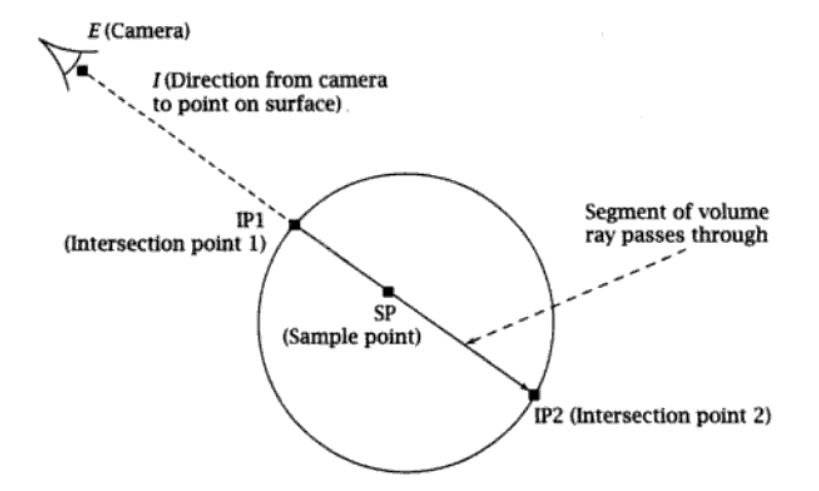
\includegraphics[width=7cm]{ray_marching.png}}
\caption{Ray marching technique for volumetric shading \cite{ray_marching}.}
\label{fig:ray_marching}
\end{figure}

\subsection{Prototype}
\begin{figure}[htbp]
\centering
\begin{subfigure}{.45\textwidth}
  \centering
  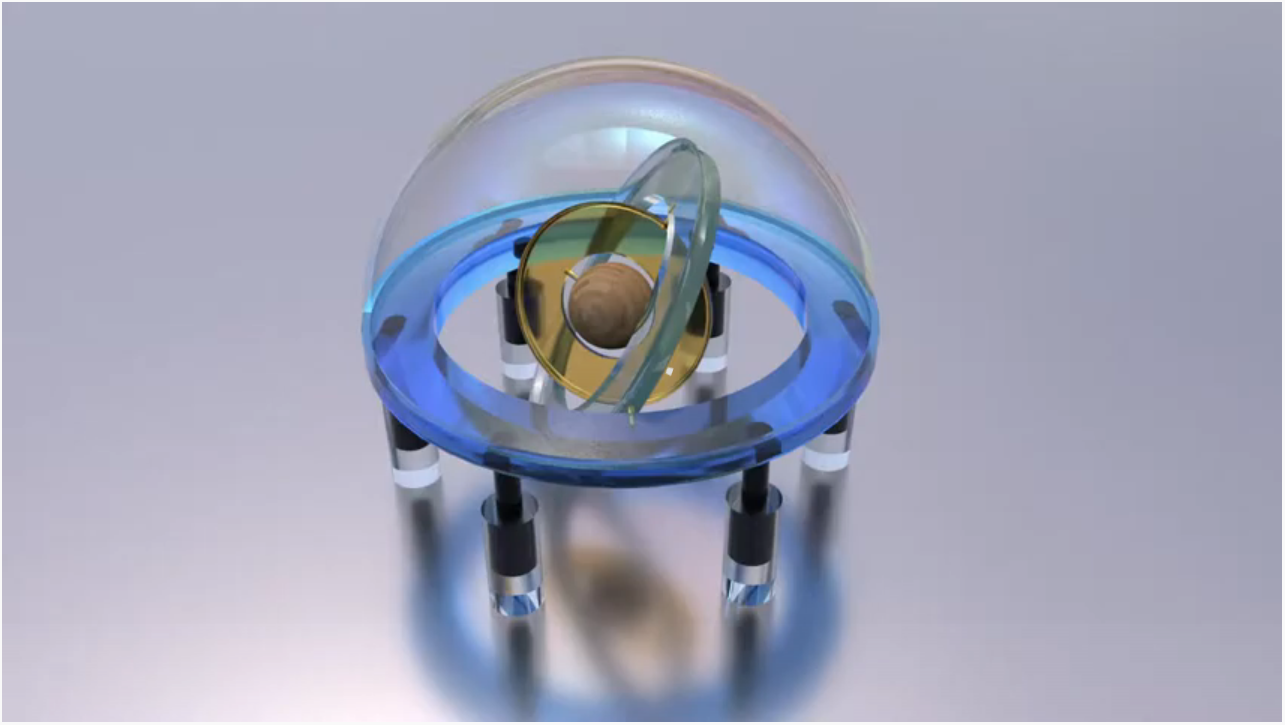
\includegraphics[width=\linewidth]{table.png}
  \caption{A realistic render of the scene using a variety of pre-built RenderMan nodes.}
  \label{fig:table}
\end{subfigure}
\par\bigskip
\begin{subfigure}{.45\textwidth}
  \centering
  
\includegraphics[width=\linewidth]{prototype_render.png}
  \caption{A render with the prototype frameblock shader using PxrConstant nodes in RenderMan.}
  \label{fig:prototype}
\end{subfigure}
\caption{``Table'' animated with Autodesk Maya and rendered with RenderMan \cite{animation}.}
\label{fig:render}
\end{figure}

A prototype system was constructed using RenderMan
and Python scripting.
New RenderMan nodes each with a custom shader were created for each object in the scene.
These nodes render a constant color, set by $r$, $g$, and $b$ variable inputs.
A Python script was then written in order to set the inputs for each shader.
The script accomplished the following:
\bigskip
\begin{enumerate}
\item Split the screen into a variable number of frameblocks.
\item Transformed all objects in the scene into screen space, using world-to-screen camera transformation.
\item Used the Cohen-Sutherland algorithm to identify if an edge of an object is inside a frameblock.
\item Parameterized screen space where $r$ lies on the $x$-axis, and $b$ on the $y$-axis.
This is shown for a frame split of 8 x 8 blocks in Figure \ref{fig:parameterization}.
\item Calculated the floating point color value for the centroid of each frameblock:
$$v : (r=\frac{(x_2 + x_1)}{2}, g=1, b=\frac{y_2 + y_1}{2})$$
\item Assigned a color value to each object, where
$F$ is the set of frameblocks the object is inside of:
$$v_{object} = \sum_{v_i\in F}v_i$$
\end{enumerate}
\bigskip
RenderMan is used to render the encoded frame.
An example render and its encoded frameblock colors are shown in Figure \ref{fig:render}.
The example shown has 64 total frame blocks spanning a rendered frame.
The bit representations of each block are discussed later.

\begin{figure}[h!]
\begin{center}
\begin{minipage}[t]{\linewidth}
\hspace{0.05\linewidth}
%\rule[-1em]{0pt}{3cm}
\begin{tikzpicture}
% R
\draw (-2,3) -- (3,3); % r horizontal line
\draw (-2,2.95) -- (-2,3.05); % r left tick
\draw (3,2.95) -- (3,3.05); % r right tick
\node[above = 1mm of {(0.5,3)}] {$r$};
%\filldraw[draw=black,fill=lightgray] (1.5,4) rectangle (3.5,4.5);
\filldraw[draw=black,fill={0,0,0}] (-2,1) rectangle (-1,2);
\filldraw[draw=black,fill={1,0,0}] (-1,1) rectangle (0,2);
%\filldraw[draw=black,fill=white] (0,1) rectangle (1,2);
\filldraw[draw=black,fill={6,0,0}] (1,1) rectangle (2,2);
\filldraw[draw=black,fill={7,0,0}] (2,1) rectangle (3,2);
\node[above = 3mm of {(-1.5,2)}] {\scriptsize{$r(1)$}};
\node[above = 0.5mm of {(-1.5,2)}] {\scriptsize{$\textbf{0x00}$}};
\node[above = 3mm of {(-0.5,2)}] {\scriptsize{$r(2)$}};
\node[above = 0.5mm of {(-0.5,2)}] {\scriptsize{$\textbf{0x02}$}};
\node[above = 3mm of {(1.5,2)}] {\scriptsize{$r(7)$}};
\node[above = 0.5mm of {(1.5,2)}] {\scriptsize{$\textbf{0x040}$}};
\node[above = 3mm of {(2.5,2)}] {\scriptsize{$r(8)$}};
\node[above = 0.5mm of {(2.5,2)}] {\scriptsize{$\textbf{0x80}$}};
% B
\draw (-3.25,2) -- (-3.25,-1); % b vertical line
\draw (-3.3,2) -- (-3.2,2); % b top tick
\draw (-3.3,-1) -- (-3.2,-1); % b bottom tick
\node[left = 2mm of {(-3.15,0.5)}] {$b$};
\filldraw[draw=black,fill={0,0,7}] (-2,-1) rectangle (-1,0);
\filldraw[draw=black,fill={1,0,7}] (-1,-1) rectangle (0,0);
%\filldraw[draw=black,fill=white] (0,-1) rectangle (1,0);
\filldraw[draw=black,fill={6,0,7}] (1,-1) rectangle (2,0);
\filldraw[draw=black,fill={7,0,7}] (2,-1) rectangle (3,0);
\node[left = 1mm of {(-2,1.69)}] {\scriptsize{$b(1)$}};
\node[left = 1mm of {(-2,1.36)}] {\scriptsize{$\textbf{0x01}$}};
\node[left = 1mm of {(-2,-0.36)}] {\scriptsize{$b(8)$}};
\node[left = 1mm of {(-2,-0.69)}] {\scriptsize{$\textbf{0x80}$}};
% Dots
\node[right = 1.75mm of {(0,1.5)}] {$\dots$};
\node[right = 1.75mm of {(0,-0.55)}] {$\dots$};
\node[right = 3mm of {(2,0.6)}] {$\vdots$};
\node[right = 3mm of {(-2,0.6)}] {$\vdots$};
\node[right = -3.5mm of {(0.5,0.6)}] {$\ddots$};
% Labels
\node[left = -2mm of {(-1.5,1.5)},fill=white] {$0$};
\node[left = -2mm of {(-0.5,1.5)},fill=white] {$1$};
\node[left = -2mm of {(1.5,1.5)},fill=white] {$6$};
\node[left = -2mm of {(2.5,1.5)},fill=white] {$7$};
\node[left = -2.75mm of {(-1.5,-0.5)},fill=white] {$56$};
\node[left = -2.75mm of {(-0.5,-0.5)},fill=white] {$57$};
\node[left = -2.95mm of {(1.5,-0.5)},fill=white] {$62$};
\node[left = -2.95mm of {(2.5,-0.5)},fill=white] {$63$};
\end{tikzpicture}
\caption{Parameterization of screen space using $r$ and $b$.}
\label{fig:parameterization}
\end{minipage}
\end{center}
\end{figure}

\section{Future Work}
\label{sec:future}
The prototype proved that the concept of frameblock shading is obtainable, however
more work is necessary for creating the full system.
The rest of the term will be focused on creating the final system and evaluating the outputs it generates.
Any extra time will be spent looking at optimizations to speed up processing and render times.

\subsection{System Architecture}
$r$ and $b$ were used to parameterize the screen
and create a map of colors to frameblocks.
However there is a problem with the current method of parameterization
and output color -- it is unknown which frameblocks make up the color
for a given object. Take for example the periwinkle-blue objects in the center of
Figure \ref{fig:prototype}. These objects have the same frameblock color, even though
some of the frameblocks are different.
The discrepency comes from using addition over the space of real values between 0 and 1;
$1 + 2 + 3$ equals $6$, but so does $3 + 3$. We need a way to uniquely map objects to a given frameblock.

Colors can range over 256 values, or 8 bits.
Let each of the 8 x 8 blocks parameterized by $r$ and $b$ each represent one bit,
as shown in Figure \ref{fig:parameterization}
(bit 0x01 was skipped since it is so close to bits 0x00 and 0x02).
Then each frameblock has a unique color-code with values of 0x00, 0x02, \dots, 0x04, 0x08.
Instead of addition, we can use a logical disjunction to OR blocks together.
The result of this is a unique color for the object representing which frameblocks contain it.
The problem we have now is that a frame can only be broken into 64 blocks.
Since our frames have the resolution of 1080 x 1920, this means each block will have
a resolution of 135 x 240. The resolution we would like is much smaller, 64 x 64
or even 32 x 32.
We can use the $g$ value to help us break the frame into smaller frameblocks.
First consider using each of the 8 bits of $g$ to overlap with one parameterized section of screen space,
as is shown in Figure \ref{fig:partition}.

\begin{figure}[h!]
\begin{center}
\begin{minipage}[t]{\linewidth}
\hspace{0.065\linewidth}
%\rule[-1em]{0pt}{0cm}
\begin{tikzpicture}
% R
\draw (-2,3) -- (0,3); % r horizontal line
\draw (-2,2.95) -- (-2,3.05); % r left tick
\draw (0,2.95) -- (0,3.05); % r right tick
\node[above = 1mm of {(-1,3)}] {$r(1..8)$};
\draw (0,3) -- (2,3); % r horizontal line
\draw (0,2.95) -- (0,3.05); % r left tick
\draw (2,2.95) -- (2,3.05); % r right tick
\node[above = 1mm of {(1,3)}] {$r(1..8)$};
%\filldraw[draw=black,fill={0,0,0}] (-2,1) rectangle (-1,2);
%\filldraw[draw=black,fill={0,1,0}] (-1,1) rectangle (0,2);
%\filldraw[draw=black,fill={0,2,0}] (0,1) rectangle (1,2);
%\filldraw[draw=black,fill={0,3,0}] (1,1) rectangle (2,2);
\node[above = 3mm of {(-1.5,2)}] {\scriptsize{$g(1)$}};
\node[above = 0.5mm of {(-1.5,2)}] {\scriptsize{$\textbf{0x00}$}};
\node[above = 3mm of {(-0.5,2)}] {\scriptsize{$g(2)$}};
\node[above = 0.5mm of {(-0.5,2)}] {\scriptsize{$\textbf{0x01}$}};
\node[above = 3mm of {(0.5,2)}] {\scriptsize{$g(3)$}};
\node[above = 0.5mm of {(0.5,2)}] {\scriptsize{$\textbf{0x02}$}};
\node[above = 3mm of {(1.5,2)}] {\scriptsize{$g(4)$}};
\node[above = 0.5mm of {(1.5,2)}] {\scriptsize{$\textbf{0x04}$}};
% B
\draw (-2.25,2) -- (-2.25,0); % b vertical line
\draw (-2.3,2) -- (-2.2,2); % b top tick
\draw (-2.3,0) -- (-2.2,0); % b bottom tick
\node[left = 2mm of {(-2.15,1)}] {$b(1..8)$};
%\filldraw[draw=black,fill={0,4,0}] (-2,0) rectangle (-1,1);
%\filldraw[draw=black,fill={0,5,0}] (-1,0) rectangle (0,1);
%\filldraw[draw=black,fill={0,6,0}] (0,0) rectangle (1,1);
%\filldraw[draw=black,fill={0,7,0}] (1,0) rectangle (2,1);
\shade[left color={7,0,1},right color={1,0,7}, shading angle=-45] (-2,1) rectangle (-1,2);
%\shade[path fading=rectangular fading, fill={7,0,7}] (-2,1) rectangle (-1,2);
\shade[left color={7,1,1},right color={1,1,7}, shading angle=-45] (-1,1) rectangle (0,2);
%\shade[path fading=rectangular fading, fill={7,0,7}] (-1,1) rectangle (0,2);
\shade[left color={7,2,1},right color={1,2,7}, shading angle=-45] (0,1) rectangle (1,2);
%\shade[path fading=rectangular fading, fill={7,0,7}] (0,1) rectangle (1,2);
\shade[left color={7,3,1},right color={1,3,7}, shading angle=-45] (1,1) rectangle (2,2);
%\shade[path fading=rectangular fading, fill={7,0,7}] (1,1) rectangle (2,2);
\shade[left color={7,4,1},right color={1,4,7}, shading angle=-45] (-2,0) rectangle (-1,1);
\shade[left color={7,5,1},right color={1,5,7}, shading angle=-45] (-1,0) rectangle (0,1);
\shade[left color={7,6,1},right color={1,6,7}, shading angle=-45] (0,0) rectangle (1,1);
\shade[left color={7,7,1},right color={1,7,7}, shading angle=-45] (1,0) rectangle (2,1);

\node[below = 3mm of {(-1.5,0)}] {\scriptsize{$g(5)$}};
\node[below = 0.5mm of {(-1.5,0)}] {\scriptsize{$\textbf{0x10}$}};
\node[below = 3mm of {(-0.5,0)}] {\scriptsize{$g(6)$}};
\node[below = 0.5mm of {(-0.5,0)}] {\scriptsize{$\textbf{0x20}$}};
\node[below = 3mm of {(0.5,0)}] {\scriptsize{$g(7)$}};
\node[below = 0.5mm of {(0.5,0)}] {\scriptsize{$\textbf{0x40}$}};
\node[below = 3mm of {(1.5,0)}] {\scriptsize{$g(8)$}};
\node[below = 0.5mm of {(1.5,0)}] {\scriptsize{$\textbf{0x80}$}};
% Labels
\node[left = -3mm of {(-1.5,1.5)},fill=white] {$64$};
\node[left = -3.5mm of {(-0.5,1.5)},fill=white] {$128$};
\node[left = -3.5mm of {(0.5,1.5)},fill=white] {$192$};
\node[left = -3.75mm of {(1.5,1.5)},fill=white] {$256$};
\node[left = -3.75mm of {(-1.5,0.5)},fill=white] {$320$};
\node[left = -3.75mm of {(-0.5,0.5)},fill=white] {$384$};
\node[left = -3.8mm of {(0.5,0.5)},fill=white] {$448$};
\node[left = -3.85mm of {(1.5,0.5)},fill=white] {$512$};
\end{tikzpicture}
\caption{Final partition of screen space, where $g$ on top of the $r$ and $b$ parameterization.}
\label{fig:partition}
\end{minipage}
\end{center}
\end{figure}

Using this model, the screen can be broken up into 2 x 4 sections, giving us $16 * 32 = 512$ frameblocks
with resolutions of 67 x 60.
This is much better resolution, however we find there is yet another problem with this
system; if an object spans multiple frameblock sections (the odds of which increases the smaller the frameblocks get),
then it is ambiguous which frameblocks are part of which frameblock section.
To demonstrate this, consider an object that is contained by 2 frameblocks, one on each side of a frameblock section.
Thus the object could have the color value:

\begin{align*}
v &= (r = \text{0x80} \wedge \text{0x01},g=\text{0x01} \wedge \text{0x02}, b=\text{0x04} \wedge \text{0x04})\\
  &= (r=\text{0x81},g=\text{0x03},b=\text{0x04})
\end{align*}

The only block value shared between the sections is $b = \text{0x04}$, however the object's color indicates that
in both sections $g = \text{0x01}$ and $g = \text{0x02}$ blocks with coordinates $(r=\text{0x80},b=\text{0x04})$ and
$(r=\text{0x01},b=\text{0x04})$ are active. Thus it appears as though the object occupies 4 blocks instead of two.
This dilemma can be solved by offsetting the domains of $g$ so that instead of covering frameblocks
$r(i)(0..8),b(i)(0..8)$,
$g_i$ covers $r_i(0..4),b_i(0..4)$.
The usecase would then be to test the value of $g$ before evaluating $r$ and $b$.
Thus divides the domain of $g$ in half, meaning we can only cover 128 frameblocks instead of 256,
with resolutions of 67 x 120.
An example calculation of the proposed system is shown in Figure \ref{fig:example}.

\begin{figure}[h!]
\centering
\begin{subfigure}{.5\textwidth}
\begin{center}
\begin{minipage}[t]{\linewidth}
\hspace{-0.025\linewidth}
%\rule[-1em]{0pt}{0cm}
\begin{tikzpicture}
% G
\draw (-3.375,1.9) -- (0,1.9); % g horizontal line
\draw (-3.375,1.85) -- (-3.375,1.95); % g left tick
\draw (0,1.85) -- (0,1.95); % g right tick
\node[above = 0.5mm of {(-1.6875,1.9)}] {$g(6)$};
\draw (0,1.9) -- (3.375,1.9); % g horizontal line
\draw (0,1.85) -- (0,1.95); % g left tick
\draw (3.375,1.85) -- (3.375,1.95); % g right tick
\node[above = 0.5mm of {(1.6875,1.9)}] {$g(7)$};
\filldraw[draw=black,fill={0,4,0}] (-3.375,-1.6875) rectangle (0,1.6875);
\filldraw[draw=black,fill={0,6,0}] (0,-1.6875) rectangle (3.375,1.6875);
% R
\draw (-3,-1.9) -- (-0.375,-1.9); % r horizontal line
\draw (-3,-1.85) -- (-3,-1.95); % r left tick
\draw (-0.375,-1.85) -- (-0.375,-1.95); % r right tick
\node[below = -0.5mm of {(-1.6875,-1.9)}] {$r(3,4)$};
\draw (0.375,-1.9) -- (3,-1.9); % r horizontal line
\draw (0.375,-1.85) -- (0.375,-1.95); % r left tick
\draw (3,-1.85) -- (3,-1.95); % r right tick
\node[below = -0.5mm of {(1.6875,-1.9)}] {$r(5,6)$};
% B
\draw (-3.6,-1.3125) -- (-3.6,1.3125); % b vertical line
\draw (-3.55,1.3125) -- (-3.65,1.3125); % b top tick
\draw (-3.55,-1.3125) -- (-3.65,-1.3125); % b bottom tick
\node[left = 0mm of {(-3.6,0)}] {$b(3,4)$};
%\filldraw[draw=black,fill=lightgray] (1.5,4) rectangle (3.5,4.5);
% Left pairs
\filldraw[draw=black,fill={0,4,2}] (-3,-1.3125) rectangle (-1.6875,0); % bottom left
\filldraw[draw=black,fill={0,4,4}] (-1.6875,-1.3125) rectangle (-0.375,1.3125); % bottom right
\filldraw[draw=black,fill={2,4,0}] (-3,0) rectangle (-1.6875,1.3125); % top left
\filldraw[draw=black,fill={4,4,0}] (-1.6875,0) rectangle (-0.375,1.3125); % top right
% Right pairs
\filldraw[draw=black,fill={0,6,2}] (0.375,-1.3125) rectangle (1.6875,0); % bottom left
\filldraw[draw=black,fill={0,6,4}] (1.6875,-1.3125) rectangle (3,1.3125); % bottom right
\filldraw[draw=black,fill={2,6,0}] (0.375,0) rectangle (1.6875,1.3125); % top left
\filldraw[draw=black,fill={4,6,0}] (1.6875,0) rectangle (3,1.3125); % top right
%% Left pairs
%\filldraw[draw=black,fill={0,4,2}] (-2,-0.875) rectangle (-1.125,0); % bottom left
%\filldraw[draw=black,fill={0,4,4}] (-1.125,-0.875) rectangle (-0.25,0.875); % bottom right
%\filldraw[draw=black,fill={2,4,0}] (-2,0) rectangle (-1.125,0.875); % top left
%\filldraw[draw=black,fill={4,4,0}] (-1.125,0) rectangle (-0.25,0.875); % top right
%% Right pairs
%\filldraw[draw=black,fill={0,6,2}] (0.25,-0.875) rectangle (1.125,0); % bottom left
%\filldraw[draw=black,fill={0,6,4}] (1.125,-0.875) rectangle (2,0.875); % bottom right
%\filldraw[draw=black,fill={2,6,0}] (0.25,0) rectangle (1.125,0.875); % top left
%\filldraw[draw=black,fill={4,6,0}] (1.125,0) rectangle (2,0.875); % top right
% Object
\filldraw[draw=black,fill={8,8,8},fill opacity=0.25] (0,0) circle (3em);
\pattern [pattern=checkerboard,pattern color={8,8,8}] (0,0) circle (3em);
%\draw[dashed] (-1.0725,-1.55) -- (-1.0725,1.55); % vertical left
%\draw[dashed] (1.0725,-1.55) -- (1.0725,1.55); % vertical right
%\draw[dashed] (-3.15,-1.075) -- (3.2,-1.075); % horizontal bottom
%\draw[dashed] (-3.15,1.075) -- (3.2,1.075); % horizontal bottom
\end{tikzpicture}
\caption{Example of an object overlapping a partition}
\label{fig:object}
\end{minipage}
\end{center}
\end{subfigure}
\par\bigskip
\begin{subfigure}{.5\textwidth}
\begin{center}
\begin{minipage}[t]{\linewidth}
\hspace{0.225\linewidth}
%\rule[-1em]{0pt}{3cm}
\begin{tikzpicture}
% Squares
%\filldraw[draw=black,fill={4,4,0}] (-4,0.25) rectangle (-0.25,2); % top left
%\filldraw[draw=black,fill={2,6,0}] (0.25,0.25) rectangle (4,2); % top right
%\filldraw[draw=black,fill={0,6,4}] (-4,-2) rectangle (-0.25,-0.25); % bottom left
%\filldraw[draw=black,fill={0,6,2}] (0.25,-2) rectangle (4,-0.25); % bottom right
\filldraw[draw=black,fill={4,4,0}] (-2.5,1) rectangle (2.5,2); % top left
\filldraw[draw=black,fill={2,6,0}] (-2.5,0) rectangle (2.5,1); % top right
\filldraw[draw=black,fill={0,6,4}] (-2.5,-1) rectangle (2.5,0); % bottom left
\filldraw[draw=black,fill={0,6,2}] (-2.5,-2) rectangle (2.5,-1); % bottom right
\draw[dashed] (-2.5,-2.5) -- (2.5,-2.5); % horizontal line
\filldraw[draw=black,fill={8,8,8}] (-2.5,-4) rectangle (2.5,-3); % bottom right
% Labels
%\node[above = 2mm of {(-2.125,2)}] {\small$(r,g,b)=\text{(0x08,0x01,0x04)}$};
%\node[above = 2mm of {(2.125,2)}] {\small$(r,g,b)=\text{(0x08,0x02,0x08)}$};
%\node[below = 2mm of {(-2.125,-2)}] {\small$(r,g,b)=\text{(0x40,0x01,0x04)}$};
%\node[below = 2mm of {(2.125,-2)}] {\small$(r,g,b)=\text{(0x40,0x02,0x08)}$};
\node[above = -3mm of {(0,1.5)},fill=white] {\small$(r,g,b)=\text{(0x08,0x20,0x04)}$}; % top
\node[above = -3mm of {(0,0.5)},fill=white] {\small$(r,g,b)=\text{(0x08,0x40,0x08)}$};
\node[above = -3mm of {(0,-0.5)},fill=white] {\small$(r,g,b)=\text{(0x10,0x20,0x04)}$};
\node[above = -3mm of {(0,-1.5)},fill=white] {\small$(r,g,b)=\text{(0x10,0x40,0x08)}$};
% Ops
\node[right = 3mm of {(2.5,1.5)},fill=white] {\large$\mathbf{\oplus}$};
\node[right = 3mm of {(2.5,0.5)},fill=white] {\large$\mathbf{\oplus}$};
\node[right = 3mm of {(2.5,-0.5)},fill=white] {\large$\mathbf{\oplus}$};
\node[right = 3mm of {(2.5,-1.5)},fill=white] {\large$\mathbf{\oplus}$};
\node[right = 3mm of {(2.5,-2.5)},fill=white] {\large$\mathbf{=}$};
% Object
\node[above = -3mm of {(0,-3.5)},fill=white] {\small$(r,g,b)=\text{(0x18,0x60,0x0B)}$};
\end{tikzpicture}
\caption{Derivation of the color for the example object.}
\label{fig:object_color}
\end{minipage}
\end{center}
\end{subfigure}
\caption{Example showing how a color is selected for an object straddling more than one frameblock.
The color of the circle is made up of the logical disjunction of color bits.}
\label{fig:example}
\end{figure}

Although there are less frameblocks, the accuracy of the colors increases for objects spanning frameblock sections.
But what happens when an object spans over more than 2 frameblock sections?
In this case frameblocks of the next section over will possibly be active when no object resides there.
Since there are already \textit{some} active frameblocks in that section, it is unlikely for the error to cause
too many complications.
If this issue does end up causing problems, we can offset it once more using the alpha channel, $a$.
Then sections would be in total 64 frameblocks apart from each other, and errors are less likely to ocurr by chance.

\subsection{Final Semantics Generation}
To conclude this project, we plan to export semantic data from the scene per frameblock.
Now that we have found a way to find if an is object inside of a frameblock,
we must decide what data on that object to collect and export.
The ways in which objects in a scene are related to each other cannot be found before rendertime.
However, if we collect enough information about each object, we should be able to discern some amount of clarity
for that object and how it interacts with others.
We propose collecting the following information for each object processed:
\bigskip
\begin{enumerate}
\item Distance to frameblock (in worldspace).
\item Distances between nearby objects.
\item Material properties.
\item Object type.
\end{enumerate}
\bigskip
Figure \ref{fig:distances} shows an example of collecting distances of objects relative to a frameblock.
All of this data is stored for each frameblock when it is exported.
We hope that in future research a machine learning algorithm can be trained to construct an image based on this information,
and that all of these frameblocks can be stitched together to form a rendered frame.

\begin{adjustwidth}{2.5em}{0pt}
\begin{figure}[h!]
\begin{center}
\begin{tikzpicture}
\coordinate (P) at (3,2);
\coordinate (Q) at (3.5,0);
\coordinate (R) at (2,-1.5);
\draw (-1.25,1) -- (-0.75,1); % Screen (top)
\draw (-1,-1) -- (-1,1); % Screen (Z)
\draw (-1.25,-1) -- (-0.75,-1); % Screen (bottom)
\draw (-1,0) -- (3,1.5); % ZP
\draw (-1,0) -- (3.5,0); % ZQ
\draw (-1,0) -- (2,-1.5); % ZR
\draw[dashed] (3,1.5) -- (2,-1.5); % PR
\draw[dashed] (3,1.5) -- (3.5,0); % PQ
\draw[dashed] (3.5,0) -- (2,-1.5); % QR
%%Labels for the vertices are typeset.
\node[below left = -2.45mm of {(3,1.5)}] {\textbullet}; % P
\node[below left = -2.35mm of {(3.5,0)}] {\textbullet}; % Q
\node[below left = -2.5mm of {(2,-1.5)}] {\textbullet}; % R
\node[right = 1mm of {(3,1.5)}] {$P_{x,y,z}$};
\node[right = 1mm of {(3.5,0)}] {$Q_{x,y,z}$};
\node[right = 1mm of {(2,-1.5)}] {$R_{x,y,z}$};
\node[right = -5mm of {(-1,-1.3)}] {$Z_{x,y,z}$};
\end{tikzpicture}
\end{center}
\caption{Relationships between points $P$, $Q$, and $R$ and frameblock with world coordinates $Z_{x,y,z}$.}
\label{fig:distances}
\end{figure}
\end{adjustwidth}

%\section{Conclusion}
%\label{sec:conclusion}

\bibliography{project}
\bibliographystyle{IEEEtran}

\onecolumn

\pagebreak

\begin{center}
\section*{Appendix}
\label{app:b}
\end{center}

\bigskip

\footnotesize{
\begin{minted}{python}
# semantics.py
import maya.cmds as cmds
import maya.OpenMaya as om
import maya.OpenMayaUI as omui
from functools import partial

##########################
#### Helper Functions ####
##########################

# Convert world space to screen space
# https://video.stackexchange.com/questions/23382/maya-python-worldspace-to-screenspace-coordinates
def worldSpaceToScreenSpace(worldPoint):
    # Find the camera
    view = omui.M3dView.active3dView()
    cam = om.MDagPath()
    view.getCamera(cam)
    camPath = cam.fullPathName()
    
    # Get the dagPath to the camera shape node to get the world inverse matrix
    selList = om.MSelectionList()
    selList.add(cam)
    dagPath = om.MDagPath()
    selList.getDagPath(0,dagPath)
    dagPath.extendToShape()
    camInvMtx = dagPath.inclusiveMatrix().inverse()

    # Use a camera function set to get projection matrix, convert the MFloatMatrix 
    # into a MMatrix for multiplication compatibility
    fnCam = om.MFnCamera(dagPath)
    mFloatMtx = fnCam.projectionMatrix()
    projMtx = om.MMatrix(mFloatMtx.matrix)

    # Multiply all together and do the normalisation
    mPoint = om.MPoint(worldPoint[0],worldPoint[1],worldPoint[2]) * camInvMtx * projMtx;
    x = (mPoint[0] / mPoint[3] / 2 + .5)
    y = (mPoint[1] / mPoint[3] / 2 + .5)

    return [x,y]

# Collect all objects in the scene using Maya ls command
# https://stackoverflow.com/questions/22794533/maya-python-array-collecting
def collectObjects(currSel):
    meshSel = []
    for xform in currSel:
        shapes = cmds.listRelatives(xform, shapes=True) # it's possible to have more than one
        if shapes != None:
            for s in shapes:
                if cmds.nodeType(s) == 'mesh':
                    meshSel.append(xform)
  
    return meshSel
    
# Test if the mesh is bounded by the coordinates
# https://boomrigs.com/blog/2016/1/12/how-to-get-mesh-vertex-position-through-maya-api
def testMesh(mesh, bounds):    
    # Store bounds
    left = bounds[0][0]
    right = bounds[0][1]
    top = bounds[1][0]
    bottom = bounds[1][1]
    
    # Get Api MDagPath for object
    activeList = om.MSelectionList()
    activeList.add(mesh)
    dagPath = om.MDagPath()
    activeList.getDagPath(0, dagPath)

    # Iterate over all the mesh vertices and get position
    mItEdge = om.MItMeshEdge(dagPath)
    while not mItEdge.isDone():
        startPoint = mItEdge.point(0, om.MSpace.kWorld)
        endPoint = mItEdge.point(1, om.MSpace.kWorld)
        
        # Return with a True value if the edge is within the boundaries
        if clippingTest(startPoint, endPoint, bounds):
            return True
                
        mItEdge.next()
    
    return False
    
# Perform the Cohen-Sutherland Clipping test using Op Codes
# https://en.wikipedia.org/wiki/Cohen%E2%80%93Sutherland_algorithm
def clippingTest(p, q, bounds):
    opCodeP = opCode(worldSpaceToScreenSpace(p), bounds)
    opCodeQ = opCode(worldSpaceToScreenSpace(q), bounds)
        
    # Trivial reject
    if (opCodeP & opCodeQ):
        return False
        
    return True

# Return the Pp Code for a given point
def opCode(p, bounds):
    code = 0
    
    # Left of clipping window
    if p[0] < bounds[0][0]:
        code = code | 1
    
    # Right of clipping window
    if p[0] > bounds[0][1]:
        code = code | 2
        
    # Above clipping window
    if p[1] < bounds[1][0]:
        code = code | 4
        
    # Below clipping window
    if p[1] > bounds[1][1]:
        code = code | 8
        
    return code

##########################
### Main Functionality ###
##########################

# Create and display menu system
def displayWindow():
    menu = cmds.window( title="Export Semantics Tool", iconName='SemanticsTool', widthHeight=(350, 400) )
    scrollLayout = cmds.scrollLayout( verticalScrollBarThickness=16 )
    cmds.flowLayout( columnSpacing=10 )
    cmds.columnLayout( cat=('both', 25), rs=10, cw=340 )
    cmds.text( label="\nThis is the \"Sematics Tool\"! This tool will generate semantics for the loaded
                      scene.\n\n", ww=True, al="left" )
    cmds.text( label="To run:\n1) Input the information in the fields below.\n2) Click \"Run\".", al="left" )
    cmds.text( '1', label='Enter the keyframe at which to start semantics generation:', al='left', ww=True )
    startTimeField = cmds.textField()
    cmds.text( '120', label='Enter the keyframe at which to end semantics generation:', al='left', ww=True )
    endTimeField = cmds.textField()
    cmds.text( '1', label='Enter the step at which to process frames:', al='left', ww=True )
    stepTimeField = cmds.textField()
    cmds.text( '1', label='Enter the dimension of frame blocks, or -1 for the whole frame:', al='left',
               ww=True )
    blockDimField = cmds.textField()
    cmds.button( label='Run', command=partial( generateSemantics, menu, startTimeField, endTimeField,
                                               stepTimeField, blockDimField ) )
    cmds.text( label="\n", al='left' )
    cmds.showWindow( menu )

def generateSemantics( menu, startTimeField, endTimeField, stepTimeField, blockDimField, *args ):
    # Grab user input and delete window
    startTime = cmds.textField(startTimeField, q=True, tx=True )
    if (startTime == ''):
        print 'WARNING: Default start time (1) used...'
        startTime = '1'
    endTime = cmds.textField(endTimeField, q=True, tx=True )
    if (endTime == ''):
        print 'WARNING: Default end time (120) used...'
        endTime = '120'
    stepTime = cmds.textField(stepTimeField, q=True, tx=True )
    if (stepTime == ''):
        print 'WARNING: Default step time (1) used...'
        stepTime = '1'
    blockDim = cmds.textField(blockDimField, q=True, tx=True )
    if (blockDim == ''):
        print 'WARNING: Default block dim (-1) used...'
        blockDim = '-1'
    cmds.deleteUI( menu, window=True )
    
    # Set up program
    resWidth = cmds.getAttr('defaultResolution.width')
    resHeight = cmds.getAttr('defaultResolution.height')
    print(resWidth, resHeight)
    blocks = []
    if int(blockDim) < 0:
        blocks.append([[0,1],[0,1]])
    else:
        for w in range(0, resWidth / int(blockDim)):
            left = (w * int(blockDim)) / float(resWidth)
            right = ((w + 1) * int(blockDim)) / float(resWidth)
            for h in range(0, resHeight / int(blockDim)):
                top = (h * int(blockDim)) / float(resHeight)
                bottom = ((h + 1) * int(blockDim)) / float(resHeight)
                
                blocks.append([[left,right],[top,bottom]])
    
    # Obtain all meshes in the scene
    currSel = cmds.ls()
    meshes = collectObjects(currSel)
    
    # Iterate over all meshes and all boundaries
    for bounds in blocks:
        print(bounds)
        for i, mesh in enumerate(meshes):
            inBounds = testMesh(mesh, bounds)
            if inBounds:
                print(mesh)
    
##########################
####### Run Script #######
##########################

# Display window
displayWindow()
\end{minted}
%==========================================================
\end{document}
%==========================================================
